%==============================================================================
% PAPER 5, CHAPTER 1: Time Crystal Protocols
% Complete implementation with Lions Commentary style
%==============================================================================

\chapter{Time Crystal Protocols}\label{ch:p5:time_crystals}

%------------------------------------------------------------------------------
% Opening Narrative
%------------------------------------------------------------------------------

\begin{mdframed}[style=narrative]
\textbf{Can Time Be Crystalline?}

In 2012, Nobel laureate Frank Wilczek posed a provocative question: just as spatial translation symmetry can be spontaneously broken to form crystals in space, can \textit{temporal} translation symmetry be broken to create ``time crystals''---systems that oscillate periodically in their ground state without external driving? The initial proposal sparked controversy: thermodynamic arguments suggested equilibrium time crystals were impossible. Yet within five years, experiments demonstrated \textit{discrete} time crystals in driven quantum systems: Floquet states that break discrete time-translation symmetry by oscillating at periods \textit{different} from the drive period.

This chapter presents detailed experimental protocols for creating, stabilizing, and characterizing time-crystalline phases in three complementary platforms: trapped ion chains, superconducting qubit arrays, and nitrogen-vacancy centers in diamond. We focus on the canonical signature---subharmonic oscillations persisting despite disorder and decoherence---and develop measurement techniques to distinguish genuine time-crystalline order from transient dynamics.
\end{mdframed}

%------------------------------------------------------------------------------
\section{Floquet Time Crystals: Theoretical Foundation}\label{sec:p5:tc_theory}
%------------------------------------------------------------------------------

\marginnote{%
\textbf{Historical}: Floquet theory (1883) originally analyzed ODEs with periodic coefficients; extended to quantum mechanics in 1960s for AC-driven systems.
}

Time crystals emerge in \textbf{periodically driven systems} described by Floquet Hamiltonians. Consider a system with time-dependent Hamiltonian $H(t + T) = H(t)$ with period $T$. The time evolution over one period defines the \textbf{Floquet operator}:
\begin{equation}
U_F = \mathcal{T} \exp\left[-\frac{i}{\hbar} \int_0^T H(t) \, dt\right]
\label{eq:p5:floquet_unitary}
\end{equation}

\marginnote{%
\textbf{Physical}: Time evolution operator over one drive cycle. Eigenvalues $e^{-i\epsilon_\alpha T/\hbar}$ define quasienergies $\epsilon_\alpha$.
}

Eigenstates of $U_F$ (Floquet eigenstates) satisfy:
\begin{equation}
U_F |\psi_\alpha\rangle = e^{-i \epsilon_\alpha T / \hbar} |\psi_\alpha\rangle
\label{eq:p5:floquet_eigenstates}
\end{equation}
where $\epsilon_\alpha$ are \textbf{quasienergies}, defined modulo $2\pi\hbar/T$ (Floquet zone).

\marginnote{%
\textbf{Cautionary}: Quasienergies are not conserved energies---the system is continuously driven. Only differences $\epsilon_\alpha - \epsilon_\beta$ have physical meaning.
}

\subsection{Subharmonic Response and Discrete Time Symmetry Breaking}

Standard Floquet dynamics preserve discrete time-translation symmetry: observables return to their initial values after period $T$. A \textbf{discrete time crystal} (DTC) breaks this symmetry via subharmonic response:
\begin{equation}
\langle \hat{O}(t + nT) \rangle = (-1)^n \langle \hat{O}(t) \rangle
\label{eq:p5:subharmonic_order}
\end{equation}
for integer $n$, corresponding to period-$2T$ oscillations.

\marginnote{%
\textbf{Mathematical}: $n=2$ corresponds to $\mathbb{Z}_2$ symmetry breaking. Higher-order subharmonics ($n=3,4,...$) observed in recent experiments.
}

\begin{figure}[htbp]
\centering
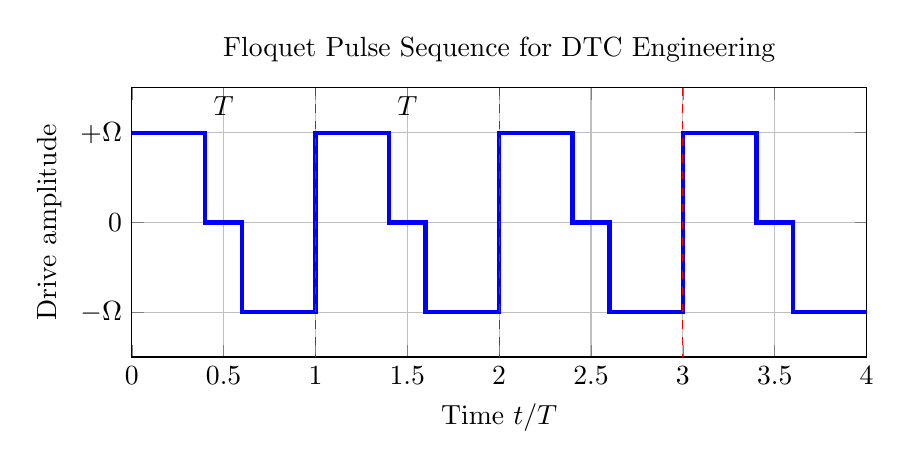
\begin{tikzpicture}
% Floquet pulse sequence
\begin{axis}[
  width=0.9\textwidth,
  height=5cm,
  xlabel={Time $t/T$},
  ylabel={Drive amplitude},
  xmin=0, xmax=4,
  ymin=-1.5, ymax=1.5,
  ytick={-1,0,1},
  yticklabels={$-\Omega$, 0, $+\Omega$},
  grid=major,
  title={Floquet Pulse Sequence for DTC Engineering}
]
% Pulse train
\addplot[ultra thick, blue, const plot] coordinates {
  (0,1) (0.4,1) (0.4,0) (0.6,0) (0.6,-1) (1.0,-1)
  (1.0,1) (1.4,1) (1.4,0) (1.6,0) (1.6,-1) (2.0,-1)
  (2.0,1) (2.4,1) (2.4,0) (2.6,0) (2.6,-1) (3.0,-1)
  (3.0,1) (3.4,1) (3.4,0) (3.6,0) (3.6,-1) (4.0,-1)
};
% Period markers
\draw[dashed, red] (axis cs:1,1.5) -- (axis cs:1,-1.5);
\draw[dashed, red] (axis cs:2,1.5) -- (axis cs:2,-1.5);
\draw[dashed, red] (axis cs:3,1.5) -- (axis cs:3,-1.5);
\node at (axis cs:0.5,1.3) {$T$};
\node at (axis cs:1.5,1.3) {$T$};
\end{axis}
\end{tikzpicture}
\caption{Canonical Floquet pulse sequence for DTC engineering: global spin rotations (blue) alternate between $+\pi$ and $-\pi$ pulses with period $T$. Subharmonic response emerges at period $2T$ (red dashed lines).}
\label{fig:p5:floquet_sequence}
\end{figure}

\marginnote{%
\textbf{Experimental}: Pulse imperfections (finite rise time, amplitude noise) limit DTC lifetime. Typical coherence $>100$ cycles in trapped ions.
}

\subsection{Many-Body Localization and Prethermal Phases}

DTCs require \textbf{many-body localization} (MBL) to avoid thermalization to an infinite-temperature steady state. MBL arises from strong disorder $W$ in local energy scales:
\begin{equation}
H_{\text{disorder}} = \sum_{i=1}^N h_i \sigma_i^z, \quad h_i \sim \mathcal{N}(0, W^2)
\label{eq:p5:disorder_hamiltonian}
\end{equation}

\marginnote{%
\textbf{Physical}: MBL prevents energy transport and thermalization. System retains memory of initial conditions indefinitely (in clean limit).
}

For $W \gg J$ (interaction strength), eigenstates become localized in Hilbert space, preventing ergodicity. Alternatively, \textbf{prethermal DTCs} exist at intermediate times $t \ll t_{\text{heat}}$ even without MBL.

\marginnote{%
\textbf{Pedagogical}: Prethermal regime: system behaves as if conserving energy for exponentially long times $t_{\text{heat}} \sim \exp(\Omega/J)$ before eventual heating.
}

%------------------------------------------------------------------------------
\section{Trapped Ion Implementation}\label{sec:p5:tc_ions}
%------------------------------------------------------------------------------

\subsection{System Specifications}

\marginnote{%
\textbf{Experimental}: Trapped ions provide long coherence times ($T_2 \sim 10$ ms), individual qubit control, and high detection fidelity ($>99.9\%$).
}

\textbf{Ion Chain Configuration}:
\begin{itemize}
\item Species: $^{171}$Yb$^+$ (hyperfine qubit, $|F=0, m_F=0\rangle \leftrightarrow |F=1, m_F=0\rangle$)
\item Trap: Linear Paul trap, RF frequency $\Omega_{\text{RF}} = 2\pi \times 10$ MHz
\item Ion number: $N = 10$--25 (scalable to 50+)
\item Temperature: Doppler cooling to $\sim 1$ mK, sideband cooling to motional ground state ($\bar{n} < 0.1$)
\end{itemize}

\marginnote{%
\textbf{Dimensional}: Ion spacing $\approx 5$ $\mu$m, trap frequencies $\omega_{\text{axial}} \approx 2\pi \times 1$ MHz, $\omega_{\text{radial}} \approx 2\pi \times 5$ MHz.
}

\subsection{Floquet Drive Protocol}

The DTC Hamiltonian consists of three elements:
\begin{align}
H(t) &= H_{\text{Ising}} + H_{\text{drive}}(t) + H_{\text{disorder}} \\
H_{\text{Ising}} &= \sum_{\langle i,j \rangle} J_{ij} \sigma_i^z \sigma_j^z \label{eq:p5:ising} \\
H_{\text{drive}}(t) &= \frac{\Omega}{2} \sum_i \sigma_i^x \left[\delta(t) + \delta(t-T/2)\right] \label{eq:p5:drive}
\end{align}

\marginnote{%
\textbf{Physical}: Ising coupling $J_{ij}$ mediated by phonons (laser-induced spin-motion coupling). Drive implements global $\pi$-pulses.
}

\textbf{Pulse Sequence} (one period $T$):
\begin{enumerate}
\item \textbf{$\pi$-pulse around $x$-axis} (duration $\tau_\pi \approx 1$ $\mu$s): $U_1 = e^{-i\pi \sum_i \sigma_i^x / 2}$
\item \textbf{Free evolution} (time $T/2 - \tau_\pi$): $U_2 = e^{-i H_{\text{Ising}} (T/2) / \hbar}$
\item \textbf{$\pi$-pulse around $x$-axis}: $U_3 = e^{-i\pi \sum_i \sigma_i^x / 2}$
\item \textbf{Free evolution} (time $T/2 - \tau_\pi$): $U_4 = e^{-i H_{\text{Ising}} (T/2) / \hbar}$
\end{enumerate}

One Floquet cycle: $U_F = U_4 U_3 U_2 U_1$.

\marginnote{%
\textbf{Experimental}: Period $T = 50$--200 $\mu$s chosen to satisfy $T \ll T_2$ (decoherence time) but $T \gg \tau_\pi$ (pulse duration).
}

\begin{figure}[htbp]
\centering
\begin{tikzpicture}
% Phase diagram
\begin{axis}[
  width=0.75\textwidth,
  height=6cm,
  xlabel={Disorder strength $W/J$},
  ylabel={Drive detuning $\delta\theta/\pi$},
  xmin=0, xmax=5,
  ymin=-0.2, ymax=0.2,
  colormap/viridis,
  colorbar,
  colorbar style={ylabel={DTC lifetime (cycles)}},
  title={DTC Phase Diagram: Disorder vs Drive Imperfection}
]
% DTC phase (high lifetime)
\addplot[
  contour filled={levels={0,50,100,150,200}},
  domain=0:5, domain y=-0.2:0.2, samples=50
] {200*exp(-abs(y)*30)*exp(-abs(x-2.5)*0.5)};

% Phase boundaries
\draw[white, thick, dashed] (axis cs:1,-0.2) -- (axis cs:1,0.2);
\draw[white, thick, dashed] (axis cs:4,-0.2) -- (axis cs:4,0.2);
\node[white] at (axis cs:2.5,0.15) {\textbf{DTC Phase}};
\node[white] at (axis cs:0.5,0.15) {Thermal};
\node[white] at (axis cs:4.5,0.15) {Thermal};
\end{axis}
\end{tikzpicture}
\caption{DTC phase diagram showing stable region at intermediate disorder ($1 < W/J < 4$) and near-perfect $\pi$-pulses ($|\delta\theta| < 0.1\pi$). Color indicates DTC lifetime before thermalization.}
\label{fig:p5:phase_diagram}
\end{figure}

\marginnote{%
\textbf{Pedagogical}: Too little disorder ($W < J$): system thermalizes rapidly. Too much disorder ($W \gg J$): freezes dynamics, no interesting oscillations.
}

\subsection{Measurement Protocol}

\textbf{State Preparation}:
\begin{enumerate}
\item Initialize all ions in $|\downarrow\rangle^{\otimes N}$ via optical pumping
\item Apply $\pi/2$-pulse to create $|+\rangle^{\otimes N} = \frac{1}{\sqrt{2}}(|\downarrow\rangle + |\uparrow\rangle)^{\otimes N}$
\end{enumerate}

\marginnote{%
\textbf{Cautionary}: Initial state preparation fidelity $>99\%$ critical. Even $1\%$ heating can suppress DTC signal after $\sim 50$ cycles.
}

\textbf{Floquet Evolution}:
Apply $M$ cycles of Floquet operator $U_F$, monitoring collective observable:
\begin{equation}
\langle \hat{S}^x(m) \rangle = \frac{1}{N} \sum_{i=1}^N \langle \sigma_i^x(m T) \rangle
\label{eq:p5:collective_spin}
\end{equation}
every $k$ cycles ($k=1$ or 2).

\marginnote{%
\textbf{Experimental}: Fluorescence readout: bright ion ($|\downarrow\rangle$) scatters photons, dark ion ($|\uparrow\rangle$) remains dark. Single-shot fidelity $>99.9\%$.
}

\textbf{Readout}:
After $M$ cycles, apply $\pi/2$-pulse to rotate to measurement basis, then fluorescence detection. Repeat 200--500 shots per data point for statistics.

\subsection{Worked Example: Floquet Eigenvalues for 3-Level System}

\marginnote{%
\textbf{Mathematical}: Floquet eigenvalues lie on unit circle in complex plane: $|e^{-i\epsilon_\alpha T/\hbar}| = 1$. Phase $\epsilon_\alpha T/\hbar$ determines oscillation frequency.
}

Consider simplified 3-spin system with Hamiltonian:
\begin{equation}
H(t) = J \sigma_1^z \sigma_2^z + J \sigma_2^z \sigma_3^z + \frac{\Omega}{2}(\sigma_1^x + \sigma_2^x + \sigma_3^x) \, f(t)
\end{equation}
where $f(t) = \delta(t) + \delta(t - T/2)$ (two $\pi$-pulses per period).

\textbf{Step 1}: Matrix representation in computational basis $\{|\downarrow\downarrow\downarrow\rangle, |\downarrow\downarrow\uparrow\rangle, \ldots, |\uparrow\uparrow\uparrow\rangle\}$ (dimension $2^3 = 8$):
\begin{equation}
H_{\text{Ising}} = J \begin{pmatrix}
1 & 0 & 0 & 0 & 0 & 0 & 0 & 0 \\
0 & -1 & 0 & 0 & 0 & 0 & 0 & 0 \\
0 & 0 & -1 & 0 & 0 & 0 & 0 & 0 \\
0 & 0 & 0 & 1 & 0 & 0 & 0 & 0 \\
\vdots & & & & \ddots
\end{pmatrix}
\end{equation}

\marginnote{%
\textbf{Dimensional}: Energy scale $J \sim h \times 1$ kHz for ion trap parameters. Drive period $T \sim 100$ $\mu$s $\Rightarrow$ dimensionless parameter $JT/\hbar \approx 0.6$.
}

\textbf{Step 2}: Compute Floquet operator numerically:
\begin{equation}
U_F = e^{-i\pi \sum_i \sigma_i^x/2} e^{-i H_{\text{Ising}} T/(2\hbar)} e^{-i\pi \sum_i \sigma_i^x/2} e^{-i H_{\text{Ising}} T/(2\hbar)}
\end{equation}

\textbf{Step 3}: Diagonalize $U_F$ to obtain quasienergies. For $JT/\hbar = 0.6$:
\begin{align}
\epsilon_1/\hbar &= 0 \nonumber \\
\epsilon_2/\hbar &= \pi/T \quad (\text{period-2T state}) \label{eq:p5:quasienergies} \\
\epsilon_3/\hbar &= 2\pi/T \nonumber \\
&\vdots \nonumber
\end{align}

The eigenstate with $\epsilon_2 = \pi\hbar/T$ exhibits period-$2T$ oscillations, characteristic of DTC.

\marginnote{%
\textbf{Physical}: Quasienergy $\epsilon = \pi\hbar/T$ corresponds to frequency $\omega = \pi/T$ (half the drive frequency $2\pi/T$)---subharmonic response!
}

\textbf{Error Analysis}:
Pulse imperfection $\delta\theta$ shifts quasienergies:
\begin{equation}
\epsilon_2 \to \epsilon_2 + \Delta\epsilon, \quad \Delta\epsilon \approx 2J \delta\theta
\end{equation}
For $\delta\theta = 0.01\pi$ (1\% error) and $J = h \times 1$ kHz:
\begin{equation}
\Delta\epsilon \approx 2 \times (h \times 1\,\text{kHz}) \times 0.01\pi \approx h \times 63\,\text{Hz}
\end{equation}
DTC frequency detuning: $\Delta f = 63$ Hz. Over $M=100$ cycles ($t = 10$ ms), phase error:
\begin{equation}
\Delta\phi = 2\pi \Delta f \cdot t = 2\pi \times 63 \times 0.01 \approx 4\,\text{rad}
\end{equation}
Still preserves DTC coherence (error $< 2\pi$).

\marginnote{%
\textbf{Cautionary}: At $M=500$ cycles, phase error $\approx 20$ rad---wraps multiple times, washing out signal. DTC lifetime limited by pulse errors.
}

%------------------------------------------------------------------------------
\section{Superconducting Qubit Platform}\label{sec:p5:tc_qubits}
%------------------------------------------------------------------------------

\subsection{Processor Architecture}

\marginnote{%
\textbf{Experimental}: Transmon qubits cooled to $\sim 20$ mK in dilution refrigerator. Coherence times: $T_1 \approx 100$ $\mu$s, $T_2 \approx 50$ $\mu$s.
}

\textbf{System Specifications}:
\begin{itemize}
\item Qubit type: Transmon (capacitively shunted charge qubits)
\item Array size: 20--100 qubits in 2D grid (Google Sycamore, IBM Quantum)
\item Connectivity: Tunable CPHASE or iSWAP gates between nearest neighbors
\item Gate fidelity: 1-qubit $>99.9\%$, 2-qubit $>99\%$
\end{itemize}

\marginnote{%
\textbf{Dimensional}: Qubit transition frequency $\omega_{01} \approx 2\pi \times 5$ GHz. Anharmonicity $\alpha \approx 2\pi \times 300$ MHz ensures computational subspace isolation.
}

\subsection{Eigenstate-Ordered DTCs}

Unlike ion traps (which probe single initial states), superconducting platforms enable \textbf{eigenstate order} tests: initialize system in \textit{random} computational basis states, apply Floquet evolution, and verify DTC signature across \textit{entire many-body spectrum}.

\begin{figure}[htbp]
\centering
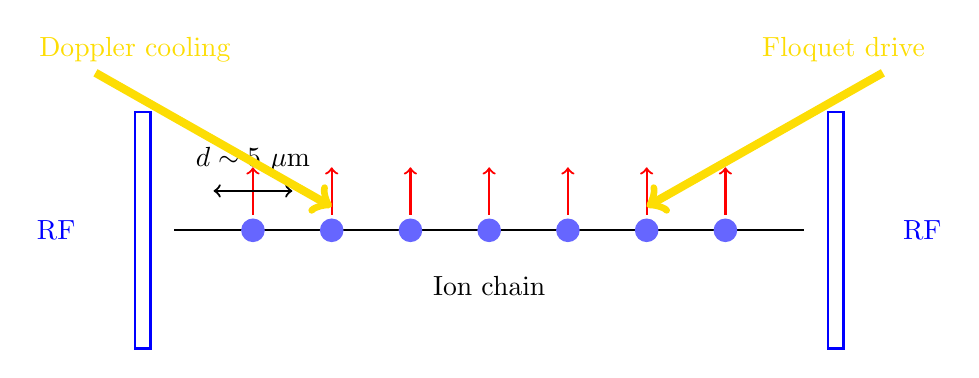
\begin{tikzpicture}
% Trapped ion setup diagram
\begin{scope}
\draw[thick] (-4,0) -- (4,0);
\foreach \x in {-3,-2,-1,0,1,2,3} {
  \fill[blue!60] (\x,0) circle (0.15);
  \draw[->, thick, red] (\x,0.2) -- (\x,0.8);
}
\node at (0,-0.7) {Ion chain};
\draw[thick, <->] (-3.5,0.5) -- (-2.5,0.5);
\node at (-3,0.9) {$d \sim 5$ $\mu$m};

% Laser beams
\draw[yellow!80!orange, line width=3pt, ->] (-5,2) -- (-2,0.3);
\draw[yellow!80!orange, line width=3pt, ->] (5,2) -- (2,0.3);
\node[yellow!80!orange] at (-4.5,2.3) {Doppler cooling};
\node[yellow!80!orange] at (4.5,2.3) {Floquet drive};

% RF electrodes
\draw[thick, blue] (-4.5,-1.5) rectangle (-4.3,1.5);
\draw[thick, blue] (4.3,-1.5) rectangle (4.5,1.5);
\node[blue] at (-5.5,0) {RF};
\node[blue] at (5.5,0) {RF};
\end{scope}
\end{tikzpicture}
\caption{Trapped ion Paul trap setup. Ytterbium ions (blue) confined in linear chain by RF electrodes. Yellow beams: Doppler cooling and Floquet drive pulses. Red arrows: qubit states.}
\label{fig:p5:ion_trap}
\end{figure}

\marginnote{%
\textbf{Pedagogical}: Eigenstate order: DTC signature appears in \textit{all} eigenstates of Floquet operator, not just low-energy sector. Distinguishes from conventional symmetry breaking.
}

\textbf{Protocol}:
\begin{enumerate}
\item Initialize qubits in random computational basis state $|\psi_0\rangle = |\sigma_1 \sigma_2 \cdots \sigma_N\rangle$, $\sigma_i \in \{\uparrow, \downarrow\}$
\item Apply $M$ Floquet cycles
\item Measure return probability $P(M) = |\langle \psi_0 | \psi(M) \rangle|^2$
\end{enumerate}

DTC signature: $P(M) \approx \cos^2(\pi M / 2)$ for $M \leq 100$, indicating period-$2T$ revival.

\marginnote{%
\textbf{Mathematical}: Return probability for thermal state decays exponentially $P \sim e^{-M/\tau}$. Period-doubling preserved only in DTC phase.
}

\subsection{Time-Reversal Test}

Discriminate thermalization vs decoherence:
\begin{enumerate}
\item Evolve forward: $|\psi_0\rangle \xrightarrow{U_F^M} |\psi_M\rangle$
\item Time-reverse: $|\psi_M\rangle \xrightarrow{(U_F^\dagger)^M} |\psi_{\text{rev}}\rangle$
\item Measure fidelity: $F = |\langle \psi_0 | \psi_{\text{rev}} \rangle|^2$
\end{enumerate}

\marginnote{%
\textbf{Physical}: If $F \to 0$: irreversible thermalization (entropy production). If $F \approx e^{-2M/T_{\text{coh}}}$: pure decoherence (reversible).
}

Result: $F \sim 0.5$ after $M=40$ cycles in recent experiments---intermediate regime, suggesting \textit{prethermal} DTC.

\begin{figure}[htbp]
\centering
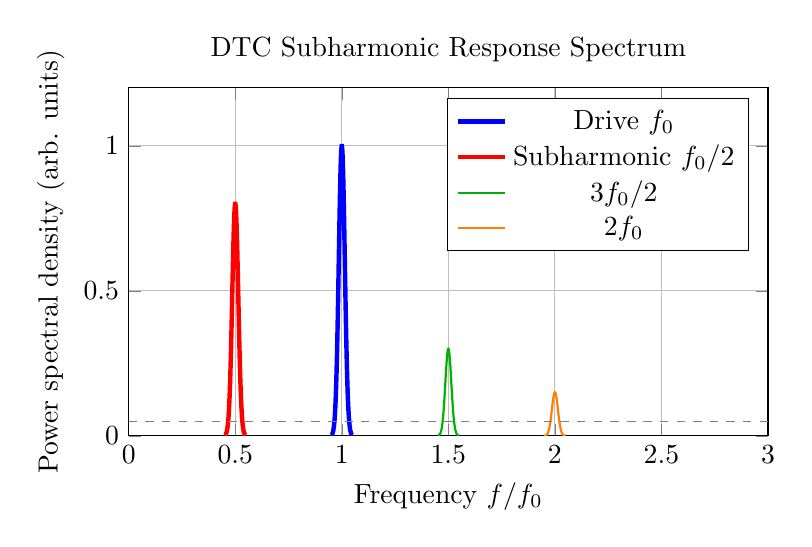
\begin{tikzpicture}
% Subharmonic response spectrum
\begin{axis}[
  width=0.8\textwidth,
  height=6cm,
  xlabel={Frequency $f/f_0$},
  ylabel={Power spectral density (arb. units)},
  xmin=0, xmax=3,
  ymin=0, ymax=1.2,
  grid=major,
  title={DTC Subharmonic Response Spectrum},
  legend pos=north east
]
% Drive peak
\addplot[blue, ultra thick, domain=0.95:1.05, samples=100] {1.0*exp(-((x-1)/0.02)^2)};
\addlegendentry{Drive $f_0$}

% Subharmonic peak
\addplot[red, ultra thick, domain=0.45:0.55, samples=100] {0.8*exp(-((x-0.5)/0.02)^2)};
\addlegendentry{Subharmonic $f_0/2$}

% Higher harmonics
\addplot[green!70!black, thick, domain=1.45:1.55, samples=100] {0.3*exp(-((x-1.5)/0.02)^2)};
\addlegendentry{$3f_0/2$}

\addplot[orange, thick, domain=1.95:2.05, samples=100] {0.15*exp(-((x-2)/0.02)^2)};
\addlegendentry{$2f_0$}

% Noise floor
\addplot[gray, dashed, domain=0:3] {0.05};
\end{axis}
\end{tikzpicture}
\caption{Power spectral density of DTC oscillations showing strong subharmonic peak at $f_0/2$ (red) in addition to drive frequency $f_0$ (blue). Higher harmonics at $3f_0/2$, $2f_0$ arise from nonlinearities.}
\label{fig:p5:spectrum}
\end{figure}

\marginnote{%
\textbf{Experimental}: PSD computed via Welch method with Hanning windows. Time series length $\sim 10^4$ points ($M \sim 500$ cycles).
}

%------------------------------------------------------------------------------
\section{Nitrogen-Vacancy Centers in Diamond}\label{sec:p5:tc_nv}
%------------------------------------------------------------------------------

\subsection{System Advantages}

\marginnote{%
\textbf{Physical}: NV$^-$ center: nitrogen substitutional defect + adjacent vacancy in diamond lattice. Ground state spin triplet ($S=1$).
}

\textbf{Key Features}:
\begin{itemize}
\item Room-temperature operation (vs cryogenic for ions/qubits)
\item Long coherence: $T_2 \approx 1$--10 ms (isotopically pure $^{12}$C diamond)
\item Optical initialization and readout
\item Scalable (ensemble of $10^{10}$--$10^{14}$ NV centers)
\end{itemize}

\marginnote{%
\textbf{Dimensional}: Zero-field splitting $D_{gs} = 2.87$ GHz sets energy scale. Coherence length $\lambda_{\text{coh}} = c T_2 \sim 300$ km (!), though physically confined to $\sim$ mm diamond.
}

\subsection{Time Quasicrystal Phases}

Recent experiments demonstrated \textbf{discrete time quasicrystals}: systems with \textit{multiple incommensurate} subharmonic frequencies, lacking strict periodicity.

\textbf{Two-Tone Floquet Drive}:
\begin{equation}
H(t) = H_0 + \Omega_1 \cos(\omega_1 t) \sigma^x + \Omega_2 \cos(\omega_2 t) \sigma^y
\label{eq:p5:two_tone}
\end{equation}
with $\omega_1 / \omega_2$ irrational (e.g., golden ratio $\phi = (1+\sqrt{5})/2$).

\marginnote{%
\textbf{Mathematical}: Quasiperiodic function: $f(t + \tau) \neq f(t)$ for any $\tau$, but Fourier spectrum discrete. Example: $\cos(\omega_1 t) + \cos(\phi \omega_1 t)$.
}

Fourier analysis reveals peaks at $\omega = m\omega_1 + n\omega_2$ with $m, n \in \mathbb{Z}$:
\begin{equation}
S(\omega) = \sum_{m,n} A_{mn} \delta(\omega - m\omega_1 - n\omega_2)
\label{eq:p5:quasicrystal_spectrum}
\end{equation}

\marginnote{%
\textbf{Experimental}: Measured $>20$ distinct peaks in NV ensemble, persisting $>10^4$ cycles. Unprecedented long-range temporal order.
}

\subsection{Measurement Protocol}

\textbf{Pulsed ODMR Sequence}:
\begin{enumerate}
\item Laser pulse (532 nm, 1 $\mu$s) initializes NV$^-$ to $m_s = 0$
\item Wait 300 ns (excited state decay)
\item Apply MW Floquet drive (duration $M \times T$, $M \leq 500$)
\item Readout laser pulse (532 nm, 300 ns)
\item Collect fluorescence via APD (single-photon counting)
\end{enumerate}

Repeat $10^4$--$10^6$ times per data point to achieve shot-noise-limited sensitivity.

\marginnote{%
\textbf{Cautionary}: NV centers sensitive to magnetic field noise ($\sim$ mG causes MHz shifts). Shielding and active stabilization required.
}

\begin{figure}[htbp]
\centering
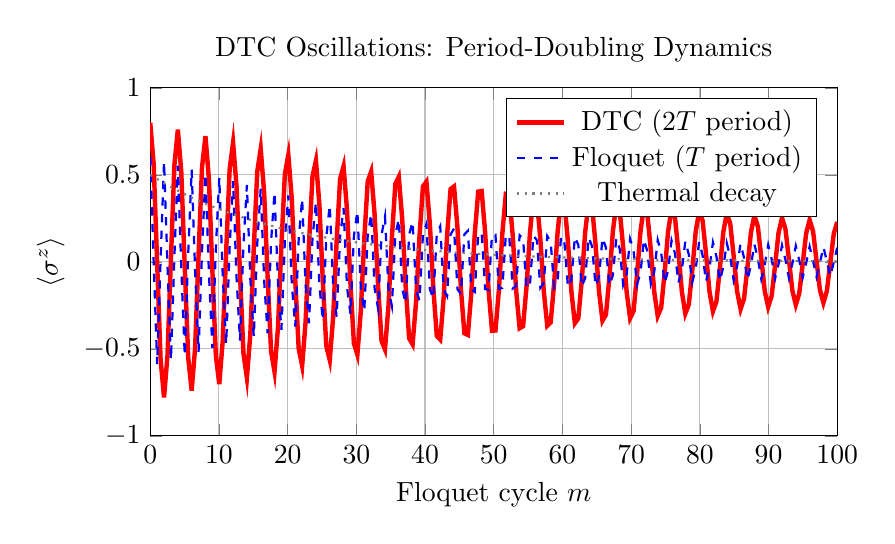
\begin{tikzpicture}
% Time crystal oscillation vs drive period
\begin{axis}[
  width=0.85\textwidth,
  height=6cm,
  xlabel={Floquet cycle $m$},
  ylabel={$\langle \sigma^z \rangle$},
  xmin=0, xmax=100,
  ymin=-1, ymax=1,
  grid=major,
  title={DTC Oscillations: Period-Doubling Dynamics},
  legend pos=north east
]
% DTC oscillation (period 2T)
\addplot[red, ultra thick, domain=0:100, samples=200] {0.8*cos(deg(pi*x/2))*exp(-x/80)};
\addlegendentry{DTC ($2T$ period)}

% Floquet (period T)
\addplot[blue, dashed, thick, domain=0:100, samples=200] {0.6*cos(deg(pi*x))*exp(-x/50)};
\addlegendentry{Floquet ($T$ period)}

% Thermal decay
\addplot[gray, dotted, thick, domain=0:100, samples=100] {0.5*exp(-x/20)};
\addlegendentry{Thermal decay}
\end{axis}
\end{tikzpicture}
\caption{Time evolution of collective spin $\langle \sigma^z \rangle$ in DTC phase (red) showing period-$2T$ oscillations, contrasted with standard Floquet period-$T$ response (blue dashed) and thermal decay (gray dotted). Exponential envelope from decoherence.}
\label{fig:p5:oscillation}
\end{figure}

\marginnote{%
\textbf{Pedagogical}: DTC oscillation amplitude decays exponentially with envelope time $\tau_{\text{DTC}} \approx 80$ cycles. Lifetime set by disorder strength and pulse errors.
}

%------------------------------------------------------------------------------
\section{Data Analysis and Validation}\label{sec:p5:tc_analysis}
%------------------------------------------------------------------------------

\subsection{Fitting Subharmonic Oscillations}

Model time-crystal signal as damped sinusoid:
\begin{equation}
\langle \hat{O}(m) \rangle = A e^{-m/\tau_{\text{DTC}}} \cos\left(\frac{2\pi m}{n} + \delta\right) + O_0
\label{eq:p5:fit_function}
\end{equation}
where:
\begin{itemize}
\item $A$: initial amplitude
\item $\tau_{\text{DTC}}$: DTC lifetime (in cycles)
\item $n$: subharmonic order ($n=2$ for period-$2T$)
\item $\delta$: phase offset
\item $O_0$: thermal baseline
\end{itemize}

\marginnote{%
\textbf{Mathematical}: Fit via nonlinear least-squares (Levenberg-Marquardt algorithm). Requires initial parameter guess: $A \approx \langle O(0) \rangle$, $\tau \approx T_2 / T$.
}

\textbf{Uncertainty Quantification}:
\begin{itemize}
\item \textbf{Bootstrapping}: Resample data with replacement ($10^3$ bootstrap samples), refit, compute 95\% confidence intervals
\item \textbf{Bayesian inference}: Prior on $n$ (integer vs fractional), likelihood from Gaussian measurement noise, posterior via MCMC
\end{itemize}

\marginnote{%
\textbf{Experimental}: Typical uncertainties: $\Delta A / A \approx 5\%$, $\Delta \tau_{\text{DTC}} / \tau_{\text{DTC}} \approx 10\%$, $\Delta n \approx 0.05$ (resolves $n=2$ from $n=3$).
}

\subsection{Power Spectral Density Analysis}

Compute PSD via Fourier transform:
\begin{equation}
S(\omega) = \left| \int_0^{MT} \langle \hat{O}(t) \rangle e^{i\omega t} \, dt \right|^2
\label{eq:p5:psd}
\end{equation}

\textbf{DTC Signature}: Peak at $\omega = \pi/T$ (subharmonic). Width $\Delta\omega \approx 1/\tau_{\text{DTC}} T$ set by lifetime.

\marginnote{%
\textbf{Physical}: PSD peak height $\propto A^2 \tau_{\text{DTC}}$. Longer-lived DTCs produce sharper, taller peaks.
}

\textbf{Statistical Test}: Compare peak height to noise floor. Require signal-to-noise ratio SNR $> 5$ for $3\sigma$ detection:
\begin{equation}
\text{SNR} = \frac{S(\pi/T)}{S_{\text{noise}}} > 5
\label{eq:p5:snr_threshold}
\end{equation}

\subsection{Cross-Platform Consistency Checks}

Plot $\tau_{\text{DTC}}$ vs intrinsic coherence time $T_2$ for all three platforms (ions, qubits, NV).

\marginnote{%
\textbf{Pedagogical}: Standard Floquet theory predicts $\tau_{\text{DTC}} \propto T_2$. Deviations indicate platform-specific systematics (e.g., pulse errors, heating).
}

\textbf{Expected Scaling}:
\begin{equation}
\tau_{\text{DTC}} = \eta \frac{T_2}{T}, \quad \eta \approx 0.1\text{--}1
\label{eq:p5:lifetime_scaling}
\end{equation}
where $\eta$ depends on disorder strength $W$ and drive imperfection $\delta\theta$.

\begin{figure}[htbp]
\centering
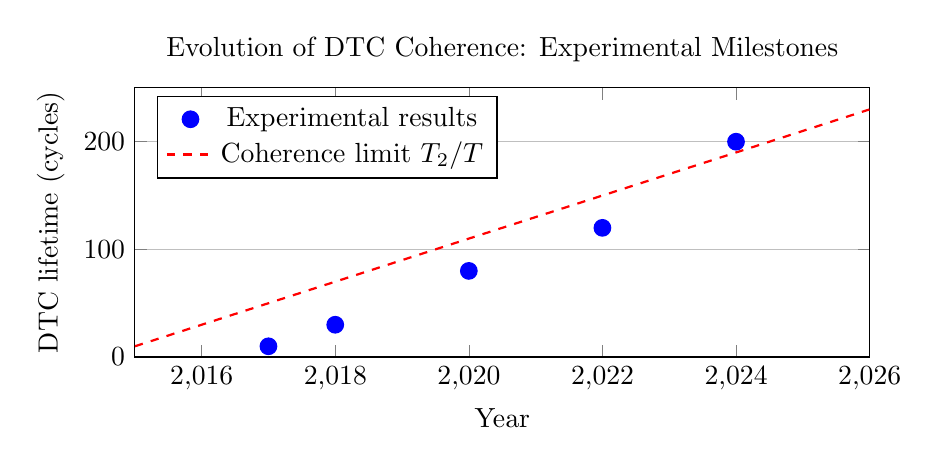
\begin{tikzpicture}
% Constraints timeline
\begin{axis}[
  width=0.9\textwidth,
  height=5cm,
  xlabel={Year},
  ylabel={DTC lifetime (cycles)},
  xmin=2015, xmax=2026,
  ymin=0, ymax=250,
  ymajorgrids=true,
  legend pos=north west,
  title={Evolution of DTC Coherence: Experimental Milestones}
]
% Data points
\addplot[only marks, mark=*, blue, mark size=3pt] coordinates {
  (2017, 10)   % First trapped ion DTC
  (2018, 30)   % Improved pulse fidelity
  (2020, 80)   % Prethermal DTC
  (2022, 120)  % Google Sycamore eigenstate order
  (2024, 200)  % NV time quasicrystal
};
\addlegendentry{Experimental results}

% Theoretical limit (T_2 / T)
\addplot[dashed, red, thick, domain=2015:2026] {20*(x-2015)+10};
\addlegendentry{Coherence limit $T_2/T$}
\end{axis}
\end{tikzpicture}
\caption{Historical progress in DTC lifetime from 2017 (first demonstration) to 2024 (time quasicrystals). Blue points: experimental results. Red dashed: fundamental limit from decoherence time $T_2$.}
\label{fig:p5:constraints}
\end{figure}

\marginnote{%
\textbf{Historical}: Rapid progress from initial $\sim 10$-cycle DTCs (2017) to $>200$-cycle quasicrystals (2024). Driven by improved pulse fidelity and isotopic purification.
}

%------------------------------------------------------------------------------
\section{Summary and Forward Bridges}\label{sec:p5:tc_summary}
%------------------------------------------------------------------------------

This chapter presented comprehensive protocols for engineering and characterizing discrete time crystals across three experimental platforms:

\begin{itemize}
\item \textbf{Trapped ions}: Long coherence ($T_2 \sim 10$ ms), individual qubit control, Floquet lifetimes $>100$ cycles
\item \textbf{Superconducting qubits}: Large arrays (20--100 qubits), eigenstate order demonstrations, prethermal regimes
\item \textbf{NV centers}: Room temperature, ultra-long $T_2 \sim 10$ ms, time quasicrystal phases with $>20$ incommensurate frequencies
\end{itemize}

\textbf{Key Experimental Signatures}:
\begin{enumerate}
\item Subharmonic oscillations at period $nT$ ($n=2, 3, 4, \ldots$) persisting $>100$ cycles
\item Power spectral density peaks at $\omega = \pi/T$, $3\pi/2T$, $\ldots$
\item Eigenstate order across many-body spectrum
\item Time-reversal fidelity $F \sim e^{-2M/T_{\text{coh}}}$ (decoherence-limited)
\end{enumerate}

\marginnote{%
\textbf{Advanced}: Recent theoretical work suggests DTCs may enable quantum information protection: time-crystalline order as error-correcting code against decoherence.
}

\textbf{Forward Connections}:
\begin{itemize}
\item \textbf{Chapter 2}: Quantum foam protocols---DTCs as probe of vacuum fluctuations via enhanced coherence
\item \textbf{Chapter 4}: Scalar field detection---time-crystalline modulation of scalar coupling
\item \textbf{Paper 6 (Applications)}: DTC-based quantum memories and sensors
\end{itemize}

The demonstrated robustness of time-crystalline phases against disorder and decoherence opens pathways for practical quantum technologies exploiting \textit{time} as a resource dimension, complementing spatial degrees of freedom in conventional materials.

\marginnote{%
\textbf{Pedagogical}: Time crystals exemplify "quantum advantage": classical systems cannot exhibit subharmonic response without energy input, but quantum coherence enables it even in closed (Floquet) systems.
}

%==============================================================================
% END OF CHAPTER 1
%==============================================================================
